\begin{figure}
  \centering
  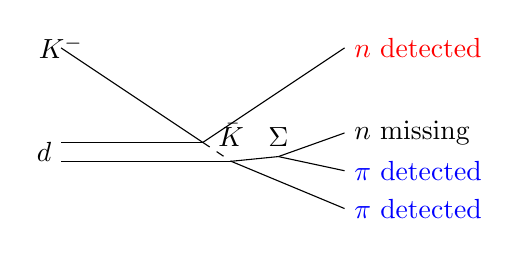
\begin{tikzpicture}[scale=1.2]
    \draw (-1.5,    1) node {$K^-$}--(0,    0);
    \draw (-1.5,    0)--(0,    0);
    \draw (-1.5, -0.2)--(0.3, -0.2);
    \node (d) at (-1.5, -0.1) [left] {$d$};

    \draw (0, 0) -- (0.3, -0.2) [dashed];
    \node (barK) at (0.3, -0.15) [above] {$\bar{K}$};

    \draw ( 1.5,  1.0) node [right] {\textcolor{red}{$n$ detected}}      -- (0,    0);
    
    \draw ( 1.5,  -0.7) node [right] {\textcolor{blue}{$\pi$ detected}} -- (0.3, -0.2);
    
    \draw ( 0.8,  -0.15) node [above] {$\Sigma$}    -- (0.3, -0.2);
    \draw ( 0.8,  -0.15) -- (1.5, 0.1) node [right] {$n$ missing};
    \draw ( 0.8,  -0.15) -- (1.5, -0.3) node [right] {\textcolor{blue}{$\pi$ detected}};    
  \end{tikzpicture}\\
  (a)
  
  \begin{tabular}{cc}
    \begin{minipage}{0.5\hsize}
      \centering
      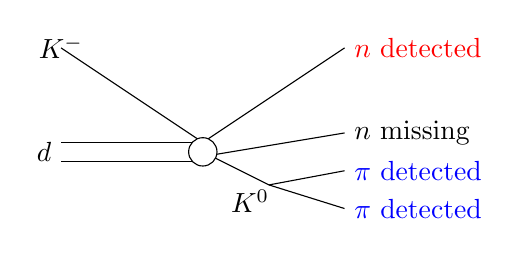
\begin{tikzpicture}[scale=1.2]
        \draw (-1.5,    1) node {$K^-$}--(0,    0);
        \draw (-1.5,    0)--(0,    0);
        \draw (-1.5, -0.2)--(0, -0.2);
        \node (d) at (-1.5, -0.1) [left] {$d$};
        
        \draw ( 1.5,  1.0) node [right] {\textcolor{red}{$n$ detected}}      -- (0,    0);

        
        \node (K0) at (0.5, -0.4) [below] {$K^0$};
        \draw (0, -0.1) -- (0.7, -0.45);
        
        \draw ( 0.0,  -0.15) -- (1.5, 0.1) node [right] {$n$ missing};
        \draw ( 0.7,  -0.45) -- (1.5, -0.3) node [right] {\textcolor{blue}{$\pi$ detected}};
        \draw (1.5,  -0.7) node [right] {\textcolor{blue}{$\pi$ detected}} -- (0.7, -0.45);
        
        \filldraw [fill=white] (0, -0.1) circle [radius=0.15];
      \end{tikzpicture}\\
      (b)
    \end{minipage}
    \begin{minipage}{0.5\hsize}
      \centering
      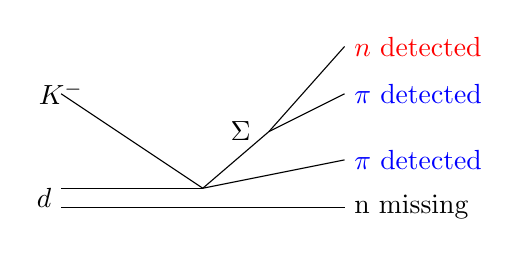
\begin{tikzpicture}[scale=1.2]
        \draw (-1.5,    1) node {$K^-$}--(0,    0);
        \draw (-1.5,    0)--(0,    0);
        \draw (-1.5, -0.2)--(0.3, -0.2);
        \node (d) at (-1.5, -0.1) [left] {$d$};

        \draw ( 1.5,  -0.2) node [right] {n missing} -- (0.3, -0.2);
        \draw ( 1.5,  0.3) node [right] {\textcolor{blue}{$\pi$ detected}}      -- (0,    0);

        \node (barK) at (0.4, 0.4) [above] {$\Sigma$};
        \draw ( 0.7,  0.6) -- (0.0, 0.0);
                
        \draw ( 0.7,  0.6) -- (1.5, 1.5) node [right] {\textcolor{red}{$n$ detected}};
        \draw ( 0.7,  0.6) -- (1.5, 1.0) node [right] {\textcolor{blue}{$\pi$ detected}};    
      \end{tikzpicture}\\
      (c)
    \end{minipage}
  \end{tabular}
  \label{fig:kd_npipin_type}
\end{figure}


The $K^- n \rightarrow n \pi^+ \pi^- n$ final state is identified from the event in which the forward neutron is detected,
as described in Section.\ref{sec:???}.
This final state can be considered to include the three reactions represented in Figure \ref{fig:kd_npipin_type}.
The first is the signal reaction in this analysis where $\bar{K}$ is recoiled backward to $\pi \Sigma$
as shown in Figure.\ref{fig:kd_npipin_type}-(a),
the second is the recoil of $K^0$ decaying directly to $\pi^+ \pi^-$ as shown in Figure \ref{fig:kd_npipin_type}-(b),
and the third is the forward production of $\Sigma$ ($\Sigma_{forward}$) as shown in Figure \ref{fig:kd_npipin_type}-(c),
where forward means that the $n$ decaying from $\Sigma$ are detected by the NC.
Reactions (b) and (c) can be identified by reconstructing $K^0$ and $\Sigma^{\pm}$
from the invariant masses of $\pi^+$ and $\pi^-$ and forward neutrons and $\pi^{\pm}$, respectively,
as shown in Figure.\ref{fig:npipin_IM_fitGauss}.
The invariant mass distributions of $\pi^+ \pi^-$, $n \pi^-$ and $n \pi^+$ are represented in the right, center and left figures respectively.
For the identification of $K^0$ and $\Sigma^{\pm}_{forward}$,
fitting with third-order polynomial function and Gaussian function is used to identify $K^0$ and $\Sigma^{\pm}_{forward}$
in the 3$\sigma$ region of the Gaussian function, which is indicated by the red hatched area.

\begin{figure}[htbp]
  \begin{tabular}{ccc}
    \begin{minipage}{0.33\hsize}
      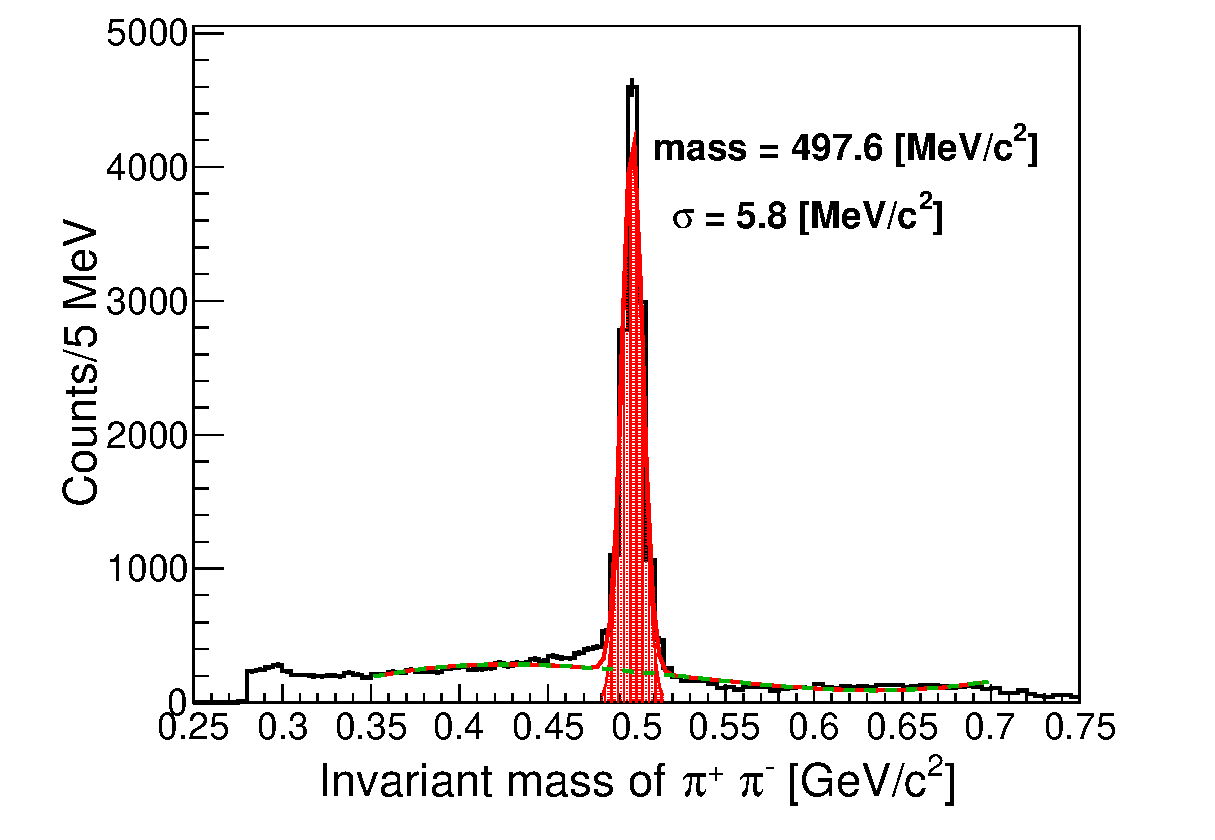
\includegraphics[width=4.5cm]{../pic/Run78/KN_ana_NC170_3sigma/IM_pipi_fitGauss.eps}
    \end{minipage}

    \begin{minipage}{0.33\hsize}
      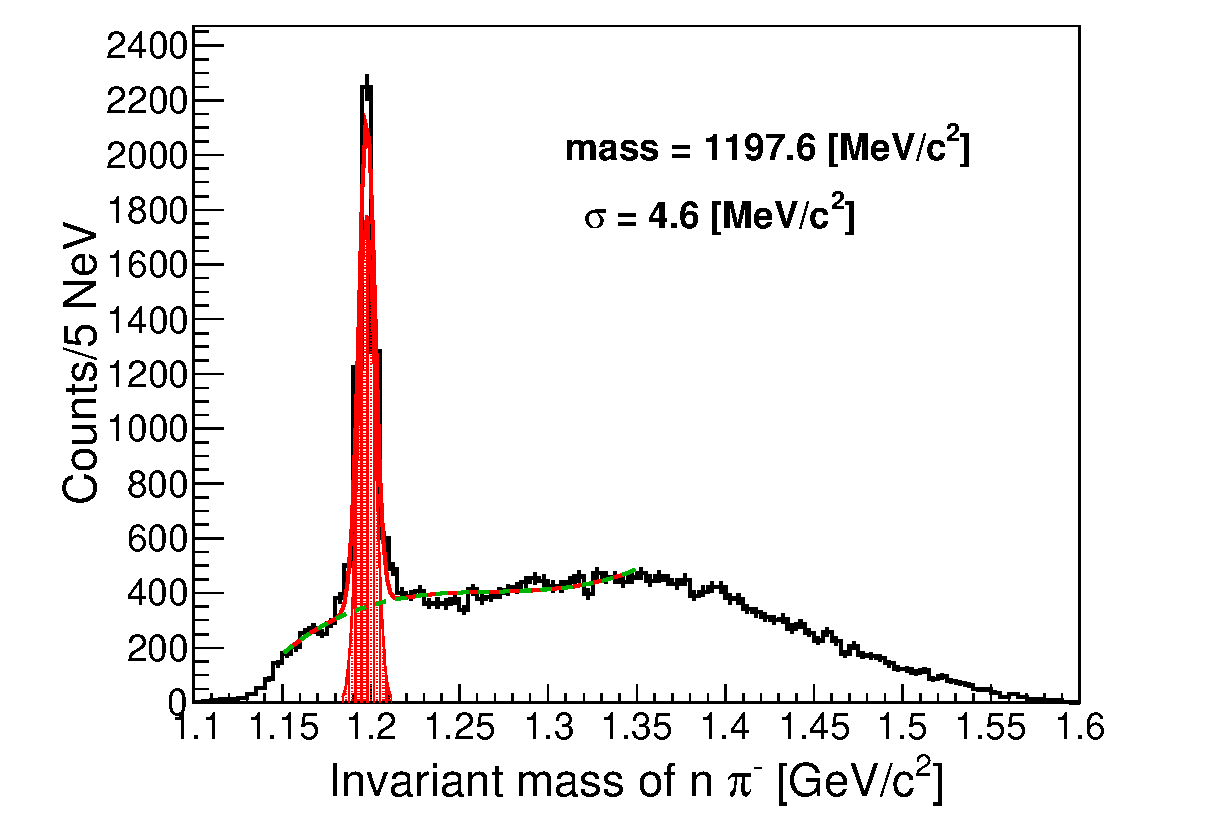
\includegraphics[width=4.5cm]{../pic/Run78/KN_ana_NC170_3sigma/IM_npim_fitGauss.eps}
    \end{minipage}

    \begin{minipage}{0.33\hsize}
      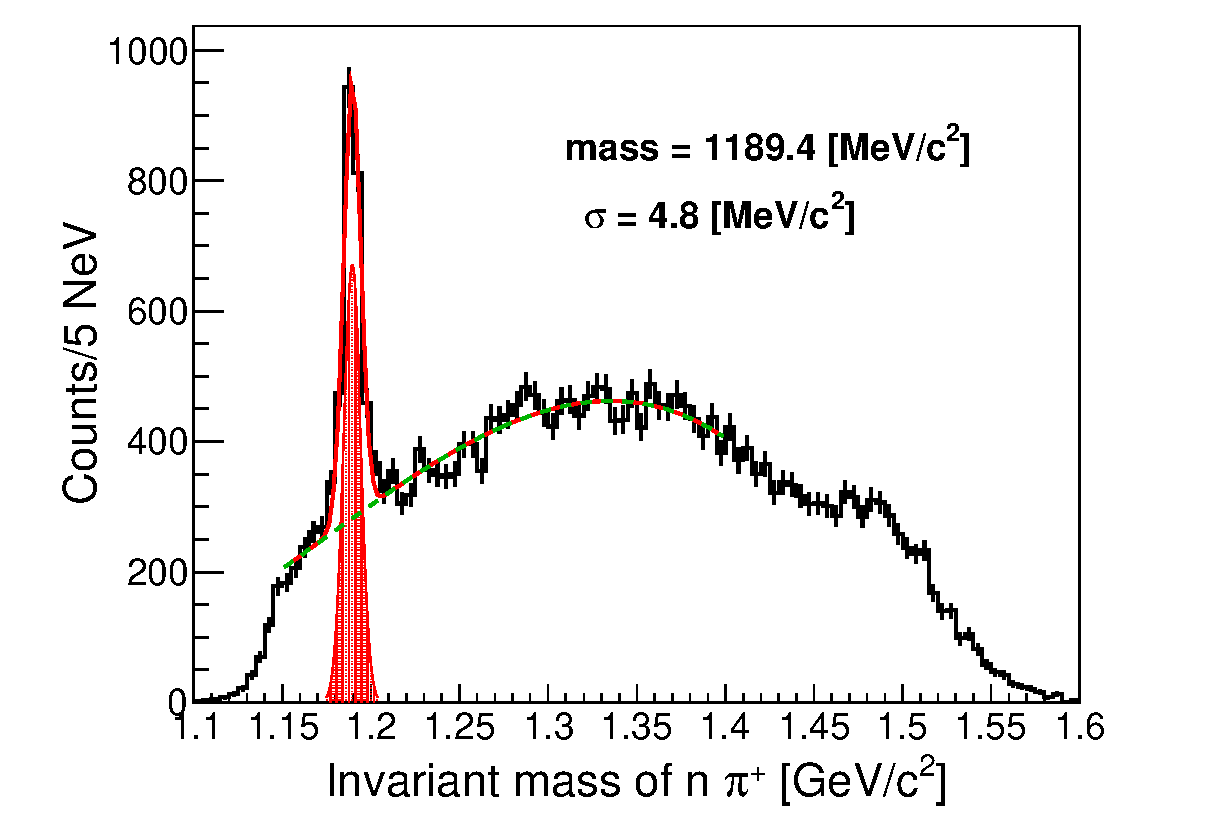
\includegraphics[width=4.5cm]{../pic/Run78/KN_ana_NC170_3sigma/IM_npip_fitGauss.eps}
    \end{minipage}
  \end{tabular}
  \caption{
    These figures show the invariant mass distributions of $\pi^+ \pi^-$,
    $n \pi^-$ and $n \pi^+$ in the $K d \rightarrow n \pi^+ \pi^- n$ event sample from left to right.
    The Gaussian functions and the selection regions for $K^0$ and $\Sigma^{\pm}_{forward}$ are indicated by red hatched area.
    The background third-order polynomial functions are shown as the green dashed lines.
  }
  \label{fig:npipin_IM_fitGauss}
\end{figure}


Rejecting these two reactions leaves a signal reaction in which $\pi \Sigma$ is scattered backward.
This reaction has $\pi^- \Sigma^+$ and $\pi^+ \Sigma^-$ modes, and they must be separated.
The branching ratio of these modes depends on the mass of $\pi \Sigma$, and this separation is performed for each bin of $d(K^-, n)$ missing mass.

\begin{frame}{$d(K^-, n)"nK0"$}
  \begin{figure}
    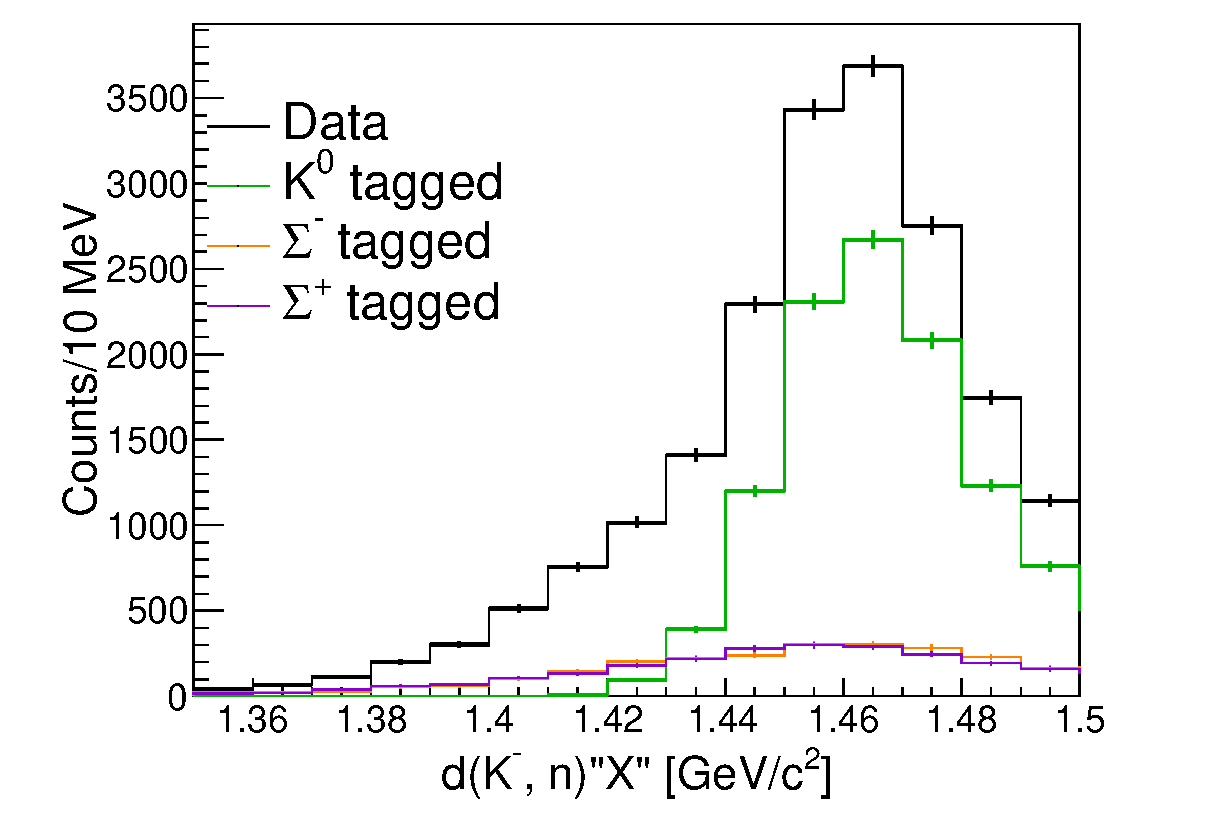
\includegraphics[width=8cm]{../pic/Run78/KN_ana_NC170_2sigma/KN_MM_all.eps}
  \end{figure}
\end{frame}


Figure \ref{fig:KN_MM_npipin} shows the $d(K^-, n)$ missing masses in which the $K^- d \rightarrow n \pi^+ \pi^- n$ final state has been identified.
On the left, all events, those identifying $K^0$, those identifying $\Sigma^+_{forward}$, and those identifying $\Sigma^-_{forward}$
are indicated by black, green, red, and blue lines, respectively.
The right figure shows the signal spectrum, subtracting the events identified as $K^0$ or $\Sigma^{\pm}_{forward}$ from all events.

To separate these events,
we generated template events using a Geant4 Monte Carlo simulation and decomposed the reactions by fitting their spectra with templates.
This decomposition was applied not only to the signal but also to the background reactions.
The procedures used in this decomposition are described in detail in Section \ref{sec:template_fitting}
The estimation of the detector resolution used in this simulation is described in detail in Appendix \ref{chapter:detector_resolution}.

